\documentclass{article}

\usepackage{siunitx} % Provides the \SI{}{} and \si{} command for typesetting SI units
\usepackage{graphicx} % Required for the inclusion of images
\usepackage{amsmath} % Required for some math elements 
\usepackage[export]{adjustbox} % loads also graphicx
\usepackage{listings}
\usepackage{matlab-prettifier}
\usepackage{float}
\usepackage[most]{tcolorbox}
\usepackage{amsfonts}
\usepackage{color}
\usepackage{titlesec}
\usepackage{caption}
\usepackage{subcaption}

\newcommand{\R}{\mathbb{R}}

\usepackage{xcolor}

\DeclareCaptionFont{white}{\color{white}}
\DeclareCaptionFormat{listing}{%
  \parbox{\textwidth}{\colorbox{gray}{\parbox{\textwidth}{#1#2#3}}\vskip-4pt}}
\captionsetup[lstlisting]{format=listing,labelfont=white,textfont=white}
\lstset{frame=lrb,xleftmargin=\fboxsep,xrightmargin=-\fboxsep}
\titleformat{\section}[runin]
  {\normalfont\Large\bfseries}{\thesection}{1em}{}
\titleformat{\subsection}[runin]
  {\normalfont\large\bfseries}{\thesubsection}{1em}{}


\setlength\parindent{0pt} % Removes all indentation from paragraphs

\renewcommand{\labelenumi}{\alph{enumi}.} % Make numbering in the enumerate environment by letter rather than number (e.g. section 6)

%\usepackage{times} % Uncomment to use the Times New Roman font

%----------------------------------------------------------------------------------------
%	DOCUMENT INFORMATION
%----------------------------------------------------------------------------------------

\title{AMATH 353: Homework 11 \\Due May, 8 2018 \\ ID: 1064712} % Title

\author{Trent \textsc{Yarosevich}} % Author name

\date{\today} % Date for the report

\begin{document}
\maketitle % Insert the title, author and date
\setlength\parindent{1cm}

\begin{center}
\begin{tabular}{l r}
%Date Performed: December 1, 2017 \\ % Date the experiment was performed
Instructor: Jeremy Upsal % Instructor/supervisor
\end{tabular}
\end{center}

% If you wish to include an abstract, uncomment the lines below
% \begin{abstract}
% Abstract text
% \end{abstract}

%----------------------------------------------------------------------------------------
%	SECTION 1
%----------------------------------------------------------------------------------------
\section*{Part 1}
This problem describes a plug flow chemical reactor of length $L$ in which a mixture of chemicals in a tube is moving from left to right with a constant speed of $c$. Inside the tube, some chemical $A$ is being turned into some other chemical based on the density at any given position, and a conversion constant $-\kappa$. The tube initially starts with a zero concentration of chemical $A$, but over time, chemical $A$ is being added to the left side of the tube such that this left edge maintains a concentration of chemical $A$ described by some function $g(t)$, and presumably $g(t)$ has a zero value at $t=0$ in order to satisfy the initial conditions.
\section*{Part 2}
This problem describes a long pipe in which a pollutant is being added to, or leaking into, the pipe at a rate of 2 units of mass per unit of time per unit of pipe length. This means that pollutant is constantly leaking into all points of the pipe at an equal rate. The initial distribution of this pollutant through the pipe is given by some function $f(x)$, and over time the pollutant diffuses from areas of higher to lower concentration at a rate relative to this change in concentration. Essentially at points of maximum concentration, the pollutant is diffusing away from that point, to the left if it is on the left of the local maximum, and to the right if it's on the right. At the extreme boundaries of the pipe, the concentration falls off to zero, which is a little at odds with the constant rate at which the pollutant is being added. A physical, real world interpretation of this could be some canal between two bodies of water, that has pollutant leaking into it everywhere at a constant rate. However, because it opens up into a larger body of water at each end, the concentration there falls off to zero as the pollutant flows out of the canal or pipe. 
\section*{Part 3}
This logarithmic relationship of traffic density and car velocity looks something like this (with arbitrarily chosen constants):
\begin{figure}[H]
  \centering
    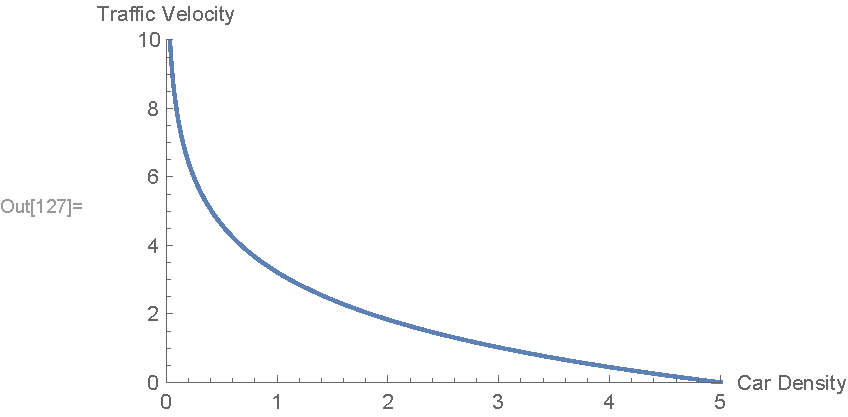
\includegraphics[width=\textwidth]{plot1.pdf}
    \caption{$\kappa = 2$ and Max car density = 5}
\end{figure}
This way of modeling differs from the linear relationship in that the traffic velocity drops off very quickly as car density begins to increase, and then more slowly as car density approaches its maximum (though both come to a standstill as maximum density is reached). I wonder if this model is more accurate because it reflects decreasing following distance as car density increases?

The resulting flux equation and conservation law with this relation are as follows:
\begin{equation}
u_t + \phi_x = 0\\
\end{equation}
\begin{tcolorbox}[minipage,colback=white,arc=0pt,outer arc=0pt]
\begin{equation}
\phi = \kappa u  \log(\frac{u_1}{u})
\end{equation}
\end{tcolorbox}
\begin{equation}
\begin{aligned}
\phi_x = \kappa\frac{d}{dx}(u\log(\frac{u_1}{u})\\
\frac{d}{dx}(u\log(\frac{u_1}{u}) = u_x\log(\frac{u_1}{u}) + u\frac{d}{dx}(\log(\frac{u_1}{u}))\\
\frac{d}{dx}\log(\frac{u_1}{u}) = \frac{u}{u_1}\frac{d}{dx}(\frac{u_1}{u})\\
\frac{d}{dx}(\frac{u_1}{u}) = \frac{-u_1}{u^2}u_x\\
\phi_x = \kappa \Big( u_x\log(\frac{u_1}{u}) + u (\frac{u}{u_1})(\frac{-u_1u_x}{u^2})\Big) \\
\phi_x = \kappa \Big( u_x\log(\frac{u_1}{u}) - u_x \Big)
\end{aligned}
\end{equation}
And finally:
\begin{tcolorbox}[minipage,colback=white,arc=0pt,outer arc=0pt]
\begin{equation}
u_t + \kappa \Big( u_x\log(\frac{u_1}{u}) - u_x \Big) = 0
\end{equation}
\end{tcolorbox}
\section*{Part 4}
By chain rule, because $\frac{d}{dt}u$ also needs to capture the information about $x(t)$'s changes over time:
\begin{equation}
\begin{aligned}
\frac{d}{dt}u(x(t), t) = u_t(x(t), t) + u_x(x(t), t)\frac{d}{dt}(x(t))\\
= u_t(x(t), t) + u_x(x(t), t)\frac{dx}{dt}
\end{aligned}
\end{equation}

\end{document}